\documentclass[aspectratio=169]{beamer}


\usetheme{metropolis}
\definecolor{pdblue}{RGB}{31,119,180}
\definecolor{pdorange}{RGB}{255,127,130}
\definecolor{pdgreen}{RGB}{44,160,44}
\definecolor{pdred}{RGB}{214,39,40}
\definecolor{pdpurple}{RGB}{148,103,189}
\definecolor{pdnavy}{RGB}{23,42,58}
\definecolor{pdfooter}{RGB}{174,195,204}
\definecolor{pdCream}{HTML}{F1F4F8}

\setbeamercolor{palette primary}{bg=pdnavy, fg=white}
\setbeamercolor{frametitle}{bg=pdnavy, fg=white}
\setbeamercolor{alerted text}{fg=pdred}
\setbeamercolor{example text}{fg=pdgreen}
\setbeamercolor{title separator}{fg=pdorange}
\metroset{progressbar=frametitle, numbering=fraction, block=fill, sectionpage=none}
\setbeamercolor{progress bar}{fg=pdorange, bg=pdnavy!15}
\setbeamercolor{block title}{bg=pdblue!20, fg=pdnavy}
\setbeamercolor{block body}{bg=pdblue!7}
\setbeamertemplate{navigation symbols}{}
\setbeamercovered{transparent}

\usepackage[utf8]{inputenc}
\usepackage[T1]{fontenc}
\usepackage{graphicx}
\usepackage[percent]{overpic}
\usepackage{tikz}
\usetikzlibrary{shapes.geometric,arrows.meta,positioning,fit,
                backgrounds,decorations.pathreplacing,calc,shadows}
\usepackage{pgfplots}
\pgfplotsset{compat=1.17}
\usepackage{booktabs}
\usepackage{hyperref}
\usepackage{algorithm2e}
\usepackage{ifthen}
\SetKwInput{KwInput}{Input}
\SetKwInput{KwOutput}{Output}
\hypersetup{colorlinks=true, linkcolor=pdorange, urlcolor=pdblue}

\title{Presentation of CSE200}
\subtitle{Participatory Design Method -- Process \& Techniques}
\author{Kazi Asef Kabir}
\institute{Department of CSE, BUET}
\date{}


\makeatletter
\setbeamertemplate{footline}{%
\begin{tikzpicture}[remember picture, overlay]
        \fill[pdnavy] (current page.south west) rectangle
                ([yshift=4.6ex]current page.south east);
                \draw[pdfooter, line width=1.2pt]
                ([yshift=4.6ex]current page.south west) -- ([yshift=4.6ex]current page.south east);
        \node[anchor=south west, xshift=0.9em, yshift=0.9ex, text=white,
                    font=\tiny\bfseries] at (current page.south west)
                        {Kazi Asef Kabir\ \textcolor{pdfooter}{\textbullet}\ \textnormal{CSE, BUET}};
                \node[anchor=south, yshift=0.9ex, text=pdfooter,
                    font=\scriptsize\itshape] at ([xshift=-1.6em]current page.south)
                    {\insertshorttitle};
        \node[anchor=south east, xshift=-0.9em, yshift=0.8ex,
                        fill=pdfooter, rounded corners=1.5pt, inner sep=2.5pt,
                    text=pdnavy, font=\scriptsize\bfseries]
                    at (current page.south east) {\insertframenumber\, /\,\inserttotalframenumber};
\end{tikzpicture}%
}
\makeatother


% =========================================================
% Reusable TikZ styles (same house style as 2305082/2305083)
% =========================================================
\tikzset{
    card/.style={
        draw=#1, thick, rounded corners=5pt, fill=#1!10,
        align=center, text=pdnavy, drop shadow
    },
    card/.default=pdblue,
    pill/.style={
        draw=#1, thick, rounded corners=9pt, fill=#1!12,
        align=center, font=\scriptsize\bfseries, text=pdnavy
    },
    pill/.default=pdblue,
    arrow/.style={
        -{Latex[length=2.5mm]}, thick, draw=pdnavy!75
    }
}

% real-image corner meme (needs the .jpg file next to this .tex when you compile)
\newcommand{\cornermeme}[3][2.3cm]{%
\begin{tikzpicture}[remember picture, overlay]
    \node[anchor=north east, xshift=-0.6em, yshift=-1.1em] at (current page.north east)
        {\begin{minipage}{#1}\centering
            \includegraphics[width=#1]{#2}\\[2pt]
            {\tiny\itshape #3}
         \end{minipage}};
\end{tikzpicture}%
}
% image files needed, so it always compiles and has no copyright risk.
% #1 = optional width (unused, kept for interface compatibility)
% #2 = mood: "facepalm" or "thumbsup" or "sweat"
% #3 = caption text
\newcommand{\tikzmeme}[3][2.2cm]{%
\begin{tikzpicture}[remember picture, overlay]
  \node[anchor=north east, xshift=-0.6em, yshift=-1.1em] at (current page.north east)
    {\begin{minipage}{#1}\centering
      \begin{tikzpicture}[scale=0.55, every node/.style={transform shape}]
        \draw[thick] (0,0) circle (0.38);
        \ifthenelse{\equal{#2}{facepalm}}{
          \draw[thick] (-0.12,-0.08) arc (160:20:0.15);
          \draw[thick] (0,-0.38) -- (0,-1.2);
          \draw[thick] (0,-0.7) -- (0.05,0.05);
          \draw[thick] (0,-0.9) -- (-0.5,-1.3);
          \draw[thick,pdblue] (0.38,0.28) .. controls (0.5,0.1) and (0.3,0.05) .. (0.38,-0.1);
        }{}
        \ifthenelse{\equal{#2}{thumbsup}}{
          \draw[thick] (-0.12,0.05) arc (200:340:0.13);
          \draw[thick] (0,-0.38) -- (0,-1.2);
          \draw[thick] (0,-0.9) -- (-0.5,-0.55);
          \fill[pdgreen] (-0.62,-0.5) circle (0.07);
          \draw[thick,pdgreen] (-0.62,-0.5) -- (-0.62,-0.3);
          \draw[thick] (0,-0.9) -- (0.4,-1.25);
        }{}
        \ifthenelse{\equal{#2}{sweat}}{
          \draw[thick] (-0.1,-0.05) circle (0.02);
          \draw[thick] (0.1,-0.05) circle (0.02);
          \draw[thick] (-0.1,-0.2) -- (0.1,-0.2);
          \draw[thick] (0,-0.38) -- (0,-1.2);
          \draw[thick] (0,-0.7) -- (-0.5,-0.9);
          \draw[thick] (0,-0.7) -- (0.5,-0.9);
          \draw[thick,pdblue] (0.3,0.3) .. controls (0.4,0.15) and (0.24,0.1) .. (0.3,-0.05);
        }{}
      \end{tikzpicture}\\[2pt]
      {\tiny\itshape #3}
     \end{minipage}};
\end{tikzpicture}%
}

\begin{document}

% ======================================================
% title (full-bleed, matches 2305082's house style)
% ======================================================
\begin{frame}[plain]
\begin{tikzpicture}[remember picture,overlay]

\fill[pdnavy] (current page.south west) rectangle (current page.north east);

\node[anchor=north west, text=white, align=left, text width=10.5cm]
  at ([xshift=1.3cm,yshift=-1.5cm]current page.north west)
{
  {\color{pdorange}\bfseries LIVE FROM THE WARD}\\[20pt]
  {\huge\bfseries Participatory Design: Process \& Techniques}
};

\draw[pdfooter!18]
  ([yshift=-1.2cm]current page.north west) --
  ([yshift=-1.2cm]current page.north east);

\begin{scope}[shift={([yshift=-1cm]current page.center)}]
\draw[pdfooter!35, line width=1.5pt] (-6,0) -- (6,0);
\foreach \x/\n in {-5/1,-3/2,-1/3,1/4,3/5,5/6}{
  \node[circle, fill=pdorange, draw=white, thick, minimum size=17pt, inner sep=0pt]
    at (\x,0) {\tiny\bfseries\color{pdnavy}\n};
}
\node[text=white, font=\tiny\bfseries, text width=1.6cm, align=center] at (-5,-0.6) {THE PROBLEM};
\node[text=white, font=\tiny\bfseries, text width=1.6cm, align=center] at (-3,-0.6) {PD SOLVES IT};
\node[text=white, font=\tiny\bfseries, text width=1.6cm, align=center] at (-1,-0.6) {PROCESS};
\node[text=white, font=\tiny\bfseries, text width=1.6cm, align=center] at (1,-0.6) {ALGORITHM};
\node[text=white, font=\tiny\bfseries, text width=1.6cm, align=center] at (3,-0.6) {TECHNIQUES};
\node[text=white, font=\tiny\bfseries, text width=1.6cm, align=center] at (5,-0.6) {INVOLVEMENT};
\end{scope}

\node[anchor=south west, xshift=1.3cm, yshift=.55cm, text=pdfooter, font=\tiny]
  at (current page.south west)
  {2305084 \quad\textcolor{pdorange}{\textbullet}\quad Kazi Asef Kabir};

\end{tikzpicture}
\end{frame}

\begin{frame}{My Part: Process \& Techniques of PD}
\centering
\vspace{.2cm}


\begin{tikzpicture}[node distance=0.7cm]
\node[pill=pdred, minimum width=2.6cm, minimum height=.75cm]
  (p1) {\normalsize PROBLEM\\[1pt]\tiny A real scenario};
\node[pill=pdgreen, minimum width=2.6cm, minimum height=.75cm, right=of p1]
  (p2) {\normalsize PROCESS\\[1pt]\tiny Four repeatable stages};
\node[pill=pdorange, minimum width=2.6cm, minimum height=.75cm, right=of p2]
  (p3) {\normalsize TECHNIQUES\\[1pt]\tiny Six concrete tools};
\node[pill=pdblue, minimum width=2.6cm, minimum height=.75cm, right=of p3]
  (p4) {\normalsize INVOLVEMENT\\[1pt]\tiny How deep to go};
\draw[arrow](p1)--(p2);
\draw[arrow](p2)--(p3);
\draw[arrow](p3)--(p4);
\end{tikzpicture}

\vspace{0.9cm}

{\Large\bfseries Goal: show \emph{how} Participatory Design\\ actually runs, step by step.}

\vspace{.3cm}
{\small\color{pdblue!40!black} From one broken hospital app to a repeatable, teachable process.}
\end{frame}

% ======================================================
% Problem Statement 
% ======================================================
\begin{frame}{The Problem -- A Real-World Scenario}
\transdissolve
\begin{center}
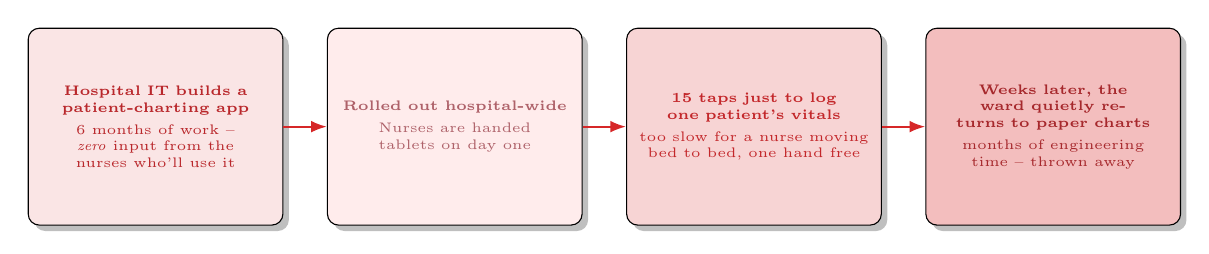
\begin{tikzpicture}[
    every node/.style={transform shape},
    sbox/.style={draw, rounded corners, fill=pdred!12, text width=3cm,
                 minimum height=2.5cm, align=center, font=\tiny, text=pdnavy, drop shadow}
]
    \node<1->[sbox, text=pdred!85!pdnavy] (s1) at (-5.7,0)
        {\textbf{Hospital IT builds a patient-charting app}\\[2pt]
        6 months of work -- \emph{zero} input from the nurses who'll use it};
    \node<2->[sbox, fill=pdorange!15, text=pdorange!65!pdnavy] (s2) at (-1.9,0)
        {\textbf{Rolled out hospital-wide}\\[2pt]
        Nurses are handed tablets on day one};
    \node<3->[sbox, fill=pdred!20, text=pdred!90!pdnavy] (s3) at (1.9,0)
        {\textbf{15 taps just to log one patient's vitals}\\[2pt]
        too slow for a nurse moving bed to bed, one hand free};
    \node<4->[sbox, fill=pdred!30, text=pdred!75!pdnavy] (s4) at (5.7,0)
        {\textbf{Weeks later, the ward quietly returns to paper charts}\\[2pt]
        months of engineering time -- thrown away};

    \draw<2->[-{Latex[length=2mm]}, thick, pdred] (s1) -- (s2);
    \draw<3->[-{Latex[length=2mm]}, thick, pdred] (s2) -- (s3);
    \draw<4->[-{Latex[length=2mm]}, thick, pdred] (s3) -- (s4);
\end{tikzpicture}
\end{center}
\vspace{0.4cm}
\onslide<5->{\centering \alert{The team never asked the one question that mattered:
\emph{``Would this actually work for the nurse holding the tablet?''}}}
\onslide<4->{\cornermeme[2.4cm]{This is fine.jpg}{Hospital IT, watching the rollout}}
\end{frame}

% ======================================================
% same scenario, resolved with Participatory Design
% ======================================================
\begin{frame}{The Same Scenario -- Solved with Participatory Design}
\begin{center}
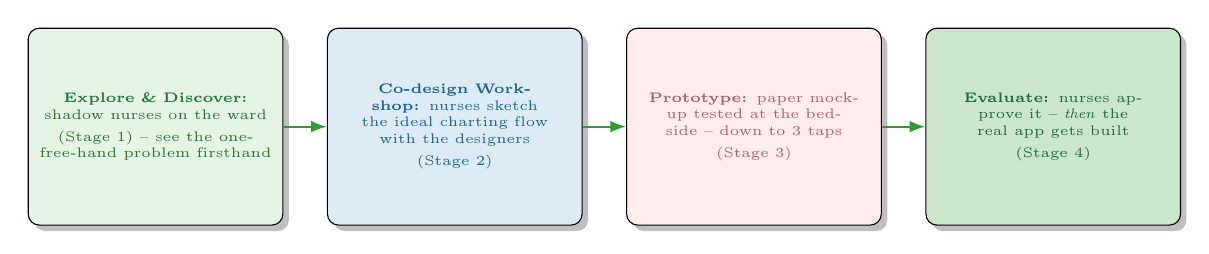
\begin{tikzpicture}[
    every node/.style={transform shape},
    gbox/.style={draw, rounded corners, fill=pdgreen!12, text width=3cm,
                 minimum height=2.5cm, align=center, font=\tiny, text=pdnavy, drop shadow}
]
    \node<1->[gbox, text=pdgreen!65!pdnavy] (g1) at (-5.7,0)
        {\textbf{Explore \& Discover:} shadow nurses on the ward\\[2pt]
        (Stage 1) -- see the one-free-hand problem firsthand};
    \node<2->[gbox, fill=pdblue!15, text=pdblue!75!pdnavy] (g2) at (-1.9,0)
        {\textbf{Co-design Workshop:} nurses sketch the ideal charting flow with
        the designers\\[2pt] (Stage 2)};
    \node<3->[gbox, fill=pdorange!15, text=pdorange!65!pdnavy] (g3) at (1.9,0)
        {\textbf{Prototype:} paper mock-up tested at the bedside -- down to 3
        taps\\[2pt] (Stage 3)};
    \node<4->[gbox, fill=pdgreen!25, text=pdgreen!55!pdnavy] (g4) at (5.7,0)
        {\textbf{Evaluate:} nurses approve it -- \emph{then} the real app gets
        built\\[2pt] (Stage 4)};

    \draw<2->[-{Latex[length=2mm]}, thick, pdgreen] (g1) -- (g2);
    \draw<3->[-{Latex[length=2mm]}, thick, pdgreen] (g2) -- (g3);
    \draw<4->[-{Latex[length=2mm]}, thick, pdgreen] (g3) -- (g4);
\end{tikzpicture}
\end{center}
\vspace{0.4cm}
\onslide<5->{\centering \alert{Same hospital, same problem -- caught and fixed
\emph{before} a single line of code was written.}}
\end{frame}

% ======================================================
% ONE flowchart replaces: cycle diagram + Stage1&2 + Stage3&4
% + algorithm slide 
% ======================================================
\begin{frame}{Solution: A Structured, Repeatable Process}
\transwipe
\begin{center}
\begin{tikzpicture}[
    node distance=0.9cm and 1.0cm,
    stage/.style={draw, rounded corners, minimum width=2.6cm, minimum height=1cm,
                  align=center, font=\small, fill=pdblue!20, drop shadow},
    dec/.style={draw, diamond, aspect=2, minimum width=3cm, minimum height=1.4cm,
                align=center, font=\small, fill=pdorange!20, drop shadow},
    every node/.style={transform shape}
]
    \node[stage] (e1) {Explore \& \\ Understand};
    \node<2->[stage, right=of e1, fill=pdorange!25] (e2) {Co-design \\ Workshops};
    \node<3->[stage, right=of e2, fill=pdgreen!25] (e3) {Prototype};
    \node<4->[dec, below=1.6cm of e3, xshift=-2.8cm] (dec) {Works for \\ users?};
    \node<5->[stage, below=0.7cm of dec, fill=pdred!20] (e4) {Implement \\ \& Evaluate};

    \draw<2->[-{Latex[length=2mm]}, thick] (e1) -- (e2);
    \draw<3->[-{Latex[length=2mm]}, thick] (e2) -- (e3);
    \draw<4->[-{Latex[length=2mm]}, thick] (e3.south) -| (dec.east);
    \draw<5->[-{Latex[length=2mm]}, thick] (dec.south) -- node[midway, right, font=\scriptsize] {Yes} (e4.north);
    \draw<5->[-{Latex[length=2mm]}, thick] (dec.west) -| node[near start, above, font=\scriptsize] {No} (e1.south);

    % ---- traveling "spotlight" ring: highlights whichever stage is currently
    % ---- active, one at a time, giving the flowchart a walked-through feel
    \begin{pgfonlayer}{background}
        \only<1>{\node[draw=pdorange, very thick, rounded corners, fit=(e1), inner sep=2.5pt] {};}
        \only<2>{\node[draw=pdorange, very thick, rounded corners, fit=(e2), inner sep=2.5pt] {};}
        \only<3>{\node[draw=pdorange, very thick, rounded corners, fit=(e3), inner sep=2.5pt] {};}
        \only<4>{\node[draw=pdorange, very thick, rounded corners, fit=(dec), inner sep=2.5pt] {};}
        \only<5>{\node[draw=pdorange, very thick, rounded corners, fit=(e4), inner sep=2.5pt] {};}
    \end{pgfonlayer}
    % ---- loop-flash: the "No" feedback path pulses red+dashed once the
    % ---- cycle is fully explained, visually emphasising the iteration
    \only<6->{\draw[-{Latex[length=2.5mm]}, ultra thick, pdred, dashed]
        (dec.west) -| node[near start, above, font=\scriptsize, text=pdred] {No -- loop!} (e1.south);}
\end{tikzpicture}
\end{center}
\onslide<5->{\centering\textit{One repeatable cycle -- restarts automatically whenever
users reject the design.}}
\begin{tikzpicture}[remember picture, overlay]
    \node[anchor=north east, xshift=-0.8em, yshift=-1.1em] at (current page.north east)
        {\begin{overpic}[width=2.3cm]{drake.jpg}
            \put(50,68){\parbox{1.4cm}{\raggedright\tiny\bfseries PD without stakeholders}}
            \put(50,18){\parbox{1.4cm}{\raggedright\tiny\bfseries PD with stakeholders}}
         \end{overpic}};
\end{tikzpicture}
\end{frame}

% ======================================================
% Algorithm
% ======================================================
\begin{frame}{The Process, Formalised as an Algorithm}
\raggedright

\small\textbf{Input:} Stakeholders $S$, Problem space $P$\\[2pt]
\textbf{Output:} Validated design $D$


\vspace{0.3cm}
\begin{tikzpicture}[
    every node/.style={font=\small, anchor=west, align=left},
    ln/.style={text width=10.3cm}
]
\node[ln] (l0) at (0,0)     {$D \gets \text{initial sketch}$};
\node[ln] (l1) at (0,-0.65)  {\textbf{while} $D$ not accepted by $S$ \textbf{do}};
\node[ln, xshift=0.6cm] (l2) at (0,-1.3)  {Explore \& gather needs from $S$};
\node[ln, xshift=0.6cm] (l3) at (0,-1.95) {Co-design $D$ together with $S$ in workshops};
\node[ln, xshift=0.6cm] (l4) at (0,-2.6)  {Build low-fidelity prototype of $D$};
\node[ln, xshift=0.6cm] (l5) at (0,-3.25) {Evaluate $D$ with $S$};
\node[ln] (l6) at (0,-3.9)   {\textbf{end}};
\node[ln] (l7) at (0,-4.55)  {\textbf{return} $D$};

% ---- program-counter style highlight: one line lights up at a time,
% ---- simulating the loop actually "running" step by step
\begin{pgfonlayer}{background}
    \only<1>{\node[fill=pdblue!25, rounded corners, fit=(l0), inner sep=3pt] {};}
    \only<2>{\node[fill=pdorange!30, rounded corners, fit=(l1), inner sep=3pt] {};}
    \only<3>{\node[fill=pdgreen!25, rounded corners, fit=(l2), inner sep=3pt] {};}
    \only<4>{\node[fill=pdgreen!25, rounded corners, fit=(l3), inner sep=3pt] {};}
    \only<5>{\node[fill=pdgreen!25, rounded corners, fit=(l4), inner sep=3pt] {};}
    \only<6>{\node[fill=pdgreen!25, rounded corners, fit=(l5), inner sep=3pt] {};}
    \only<7>{\node[fill=pdorange!30, rounded corners, fit=(l6), inner sep=3pt] {};}
    \only<8->{\node[fill=pdred!25, rounded corners, fit=(l7), inner sep=3pt] {};}
\end{pgfonlayer}

% ---- loop-back arrow appears once we've walked through one full pass,
% ---- showing the "while" actually cycles back to the top
\only<7->{\draw[-{Latex[length=2.5mm]}, thick, pdred, dashed]
    (l6.west) to[out=180, in=180] node[left, font=\scriptsize, text=pdred] {repeat} (l1.west);}
\end{tikzpicture}

\vspace{0.25cm}
\onslide<8->{\textit{Formalising the loop shows PD is systematic, not just
``brainstorming.''}}
\onslide<8->{\cornermeme[2.4cm]{cat.jpg}{Developer's life now depends on ``STAKEHOLDERS''}}
\end{frame}

% ======================================================
% ONE icon-grid slide replaces: Workshops, Surveys, Prototyping,
% Techniques 
% ======================================================
\begin{frame}{Solution: Concrete Techniques for Each Stage}
\transboxin
\begin{center}
\begin{tikzpicture}[
    every node/.style={transform shape},
    tbox/.style={draw, rounded corners, minimum width=3.5cm, minimum height=1.3cm,
                 align=center, font=\scriptsize, text=pdnavy, drop shadow}
]
    \node<1->[tbox, fill=pdblue!20, text=pdblue!80!pdnavy]   (t1) at (0,3)   {\textbf{Workshops}\\Group idea exchange};
    \node<2->[tbox, fill=pdorange!20, text=pdorange!65!pdnavy] (t2) at (5.5,3) {\textbf{Surveys \& Interviews}\\Probe needs \& pain points};
    \node<3->[tbox, fill=pdgreen!20, text=pdgreen!65!pdnavy]  (t3) at (11,3)  {\textbf{Prototyping}\\Make ideas tangible};
    \node<4->[tbox, fill=pdred!20, text=pdred!80!pdnavy]    (t4) at (0,0.5)   {\textbf{Storytelling}\\Realistic user scenarios};
    \node<5->[tbox, fill=pdpurple!20, text=pdpurple!75!pdnavy] (t5) at (5.5,0.5) {\textbf{Journey Mapping}\\Visualize start-to-finish};
    \node<6->[tbox, fill=pdblue!35, text=pdblue!85!pdnavy]   (t6) at (11,0.5)  {\textbf{Contextual Inquiry}\\Observe users in context};

    % ---- spotlight cycle: once all six are on screen, a bright ring
    % ---- sweeps across them one at a time, like a highlighter reel
    \begin{pgfonlayer}{background}
        \only<7>{\node[draw=pdorange, ultra thick, rounded corners, fit=(t1), inner sep=2pt] {};}
        \only<8>{\node[draw=pdorange, ultra thick, rounded corners, fit=(t2), inner sep=2pt] {};}
        \only<9>{\node[draw=pdorange, ultra thick, rounded corners, fit=(t3), inner sep=2pt] {};}
        \only<10>{\node[draw=pdorange, ultra thick, rounded corners, fit=(t4), inner sep=2pt] {};}
        \only<11>{\node[draw=pdorange, ultra thick, rounded corners, fit=(t5), inner sep=2pt] {};}
        \only<12>{\node[draw=pdorange, ultra thick, rounded corners, fit=(t6), inner sep=2pt] {};}
    \end{pgfonlayer}
\end{tikzpicture}
\end{center}
\onslide<13->{\centering \alert{PICTIVE} \textit{-- a shared physical kit (cards,
cut-outs) that lets any workshop turn ideas into a layout on the table.}}
\end{frame}

% ======================================================
% Choosing a technique 
% ======================================================
\begin{frame}{Solution: Right Technique, Right Stage}
\begin{center}
\begin{tabular}{@{}ll@{}}
\toprule
\textbf{Process stage} & \textbf{Best-fit technique} \\
\midrule
Explore \& Discover & Contextual interviews, shadowing \\
Co-design Workshops & PICTIVE, card sorting \\
Prototype & Personas-driven low-fidelity mock-ups \\
Evaluate & Think-aloud usability walkthroughs \\
\bottomrule
\end{tabular}
\end{center}
\end{frame}

% ======================================================
% ONE annotated chart replaces: ladder chart + "What Each Rung" text
% ======================================================
\begin{frame}{Solution: How Deep Should Users Be Involved?}
\transglitter
\begin{center}
\only<1>{%
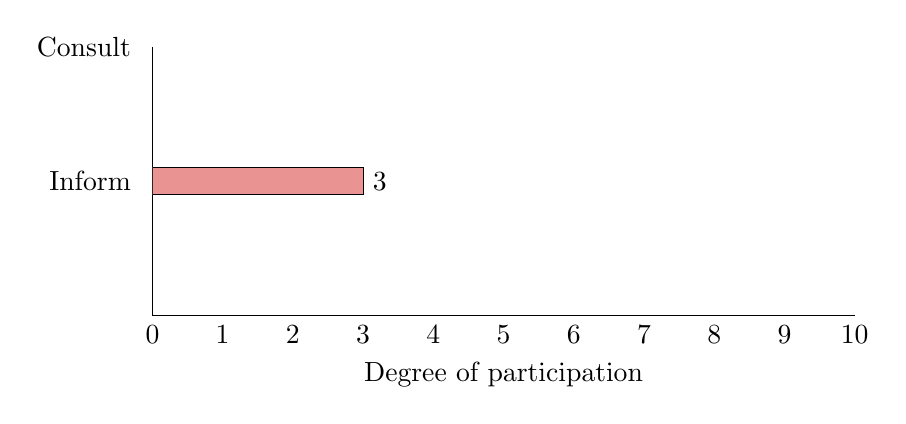
\begin{tikzpicture}
    \begin{axis}[
        xbar, width=10.5cm, height=5cm,
        xmin=0, xmax=10,
        symbolic y coords={Inform, Consult, Co-design},
        ytick={Inform, Consult, Co-design},
        enlarge y limits=0.25,
        nodes near coords, nodes near coords align={horizontal},
        axis lines*=left, tick style={draw=none},
        xlabel={Degree of participation}
    ]
    \addplot[fill=pdred!50]    coordinates {(3,Inform)};
    \end{axis}
\end{tikzpicture}}%
\only<2>{%
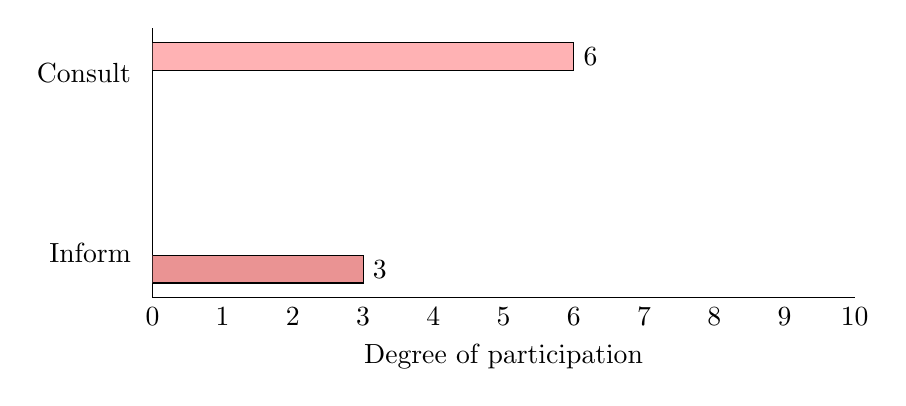
\begin{tikzpicture}
    \begin{axis}[
        xbar, width=10.5cm, height=5cm,
        xmin=0, xmax=10,
        symbolic y coords={Inform, Consult, Co-design},
        ytick={Inform, Consult, Co-design},
        enlarge y limits=0.25,
        nodes near coords, nodes near coords align={horizontal},
        axis lines*=left, tick style={draw=none},
        xlabel={Degree of participation}
    ]
    \addplot[fill=pdred!50]    coordinates {(3,Inform)};
    \addplot[fill=pdorange!60] coordinates {(6,Consult)};
    \end{axis}
\end{tikzpicture}}%
\only<3->{%
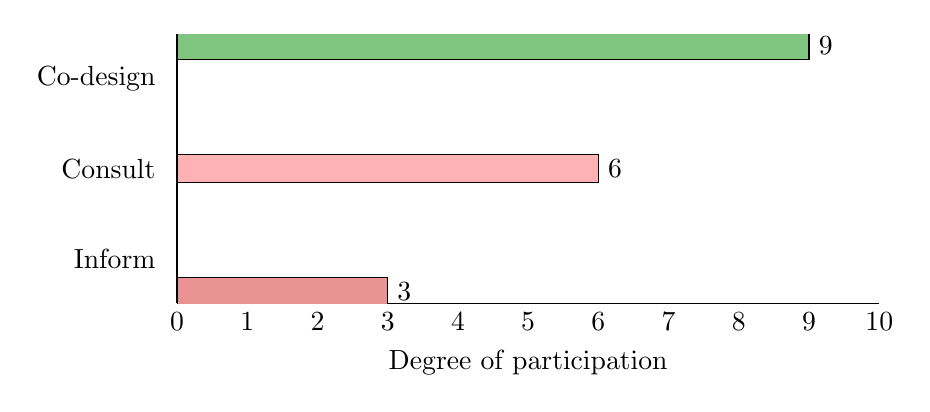
\begin{tikzpicture}
    \begin{axis}[
        xbar, width=10.5cm, height=5cm,
        xmin=0, xmax=10,
        symbolic y coords={Inform, Consult, Co-design},
        ytick={Inform, Consult, Co-design},
        enlarge y limits=0.25,
        nodes near coords, nodes near coords align={horizontal},
        axis lines*=left, tick style={draw=none},
        xlabel={Degree of participation}
    ]
    \addplot[fill=pdred!50]    coordinates {(3,Inform)};
    \addplot[fill=pdorange!60] coordinates {(6,Consult)};
    \addplot[fill=pdgreen!60]  coordinates {(9,Co-design)};
    \end{axis}
\end{tikzpicture}}%
\end{center}
\onslide<3->{\alert{\centering Participatory Design lives at the \textbf{Co-design} end of the
spectrum.}}
\end{frame}

% ======================================================
% Summary 
% ======================================================
\begin{frame}{Problem $\rightarrow$ Solved}
\begin{center}
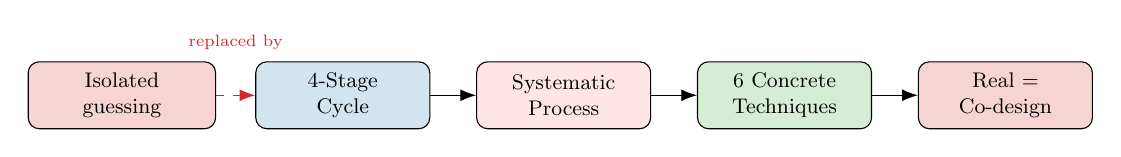
\begin{tikzpicture}[scale=0.85, every node/.style={font=\small, align=center, transform shape}]
    \node[draw, rounded corners, fill=pdred!20, minimum width=2.8cm, minimum height=1cm] (x) at (-4,0) {Isolated \\ guessing};
    \node[draw, rounded corners, fill=pdblue!20, minimum width=2.6cm, minimum height=1cm] (a) at (-0.7,0) {4-Stage\\Cycle};
    \node[draw, rounded corners, fill=pdorange!20, minimum width=2.6cm, minimum height=1cm] (b) at (2.6,0) {Systematic\\Process};
    \node[draw, rounded corners, fill=pdgreen!20, minimum width=2.6cm, minimum height=1cm] (c) at (5.9,0) {6 Concrete\\Techniques};
    \node[draw, rounded corners, fill=pdred!20, minimum width=2.6cm, minimum height=1cm] (d) at (9.2,0) {Real = \\ Co-design};
    \draw[-{Latex[length=2mm]}, dashed, pdred] (x) --
        node[midway, above=0.55cm, font=\scriptsize, text=pdred]{replaced by} (a);
    \draw[-{Latex[length=2mm]}] (a) -- (b);
    \draw[-{Latex[length=2mm]}] (b) -- (c);
    \draw[-{Latex[length=2mm]}] (c) -- (d);
\end{tikzpicture}
\end{center}
\vfill
\centering \alert{Participatory Design turns the original problem -- designing blind
for users -- into a repeatable process of designing with them.}\\[0.2cm]
\textit{Next: Tajrian will cover real-world applications, Benefits, Challenges and
wrap up with our conclusions.}
\end{frame}

% ======================================================
% Full-bleed takeaway (matches 2305082's closing style)
% ======================================================
\begin{frame}[plain]
\begin{tikzpicture}[remember picture,overlay]
\fill[pdnavy] (current page.south west) rectangle (current page.north east);

\node[anchor=center, yshift=1cm] at (current page.center)
{
\begin{minipage}{12.5cm}\centering
{\small\color{pdorange}\bfseries THE CENTRAL TAKEAWAY}\\[12pt]
{\Huge\bfseries\color{white} DESIGNING BLIND}\\[7pt]
{\Large\color{pdfooter} becomes}\\[7pt]
{\Huge\bfseries\color{pdorange} A REPEATABLE PROCESS}
\end{minipage}
};

\node[anchor=center, yshift=-1.5cm, text width=11.5cm, align=center]
  at (current page.center)
{\large\itshape\color{pdfooter}
``Formalising Participatory Design as a process turns good intentions
into something a team can actually repeat.''};

\node[anchor=south, yshift=.8cm, text=white, font=\scriptsize\bfseries]
  at (current page.south)
  {CSE200 \quad\textcolor{pdorange}{\textbullet}\quad Participatory Design};
\end{tikzpicture}
\end{frame}

% ======================================================
% Thank you (matches 2305082's closer)
% ======================================================
\begin{frame}[plain]
\begin{tikzpicture}[remember picture,overlay]
\fill[pdCream] (current page.south west) rectangle (current page.north east);

\node[anchor=center, yshift=1cm, text=pdnavy, align=center]
  at (current page.center)
{
{\Huge\bfseries THANK YOU}\\[8pt]
{\Large\color{pdnavy} for listening}
};

\draw[pdnavy, line width=1.5pt]
  ([xshift=-2.5cm,yshift=-.35cm]current page.center) --
  ([xshift=2.5cm,yshift=-.35cm]current page.center);

\node[anchor=south, yshift=.8cm, text=pdfooter, font=\scriptsize\bfseries]
  at (current page.south)
  {\small\color{pdnavy}\bfseries 2305084 \quad\textcolor{pdnavy}{\textbullet}\quad
   \small\color{pdnavy}\bfseries CSE200 \quad\textbullet\quad PARTICIPATORY DESIGN};
\end{tikzpicture}
\end{frame}

\end{document}